\documentclass[color=usenames,dvipsnames]{beamer}\usepackage[]{graphicx}\usepackage[]{color}
% maxwidth is the original width if it is less than linewidth
% otherwise use linewidth (to make sure the graphics do not exceed the margin)
\makeatletter
\def\maxwidth{ %
  \ifdim\Gin@nat@width>\linewidth
    \linewidth
  \else
    \Gin@nat@width
  \fi
}
\makeatother

\definecolor{fgcolor}{rgb}{0.345, 0.345, 0.345}
\newcommand{\hlnum}[1]{\textcolor[rgb]{0.686,0.059,0.569}{#1}}%
\newcommand{\hlstr}[1]{\textcolor[rgb]{0.192,0.494,0.8}{#1}}%
\newcommand{\hlcom}[1]{\textcolor[rgb]{0.678,0.584,0.686}{\textit{#1}}}%
\newcommand{\hlopt}[1]{\textcolor[rgb]{0,0,0}{#1}}%
\newcommand{\hlstd}[1]{\textcolor[rgb]{0.345,0.345,0.345}{#1}}%
\newcommand{\hlkwa}[1]{\textcolor[rgb]{0.161,0.373,0.58}{\textbf{#1}}}%
\newcommand{\hlkwb}[1]{\textcolor[rgb]{0.69,0.353,0.396}{#1}}%
\newcommand{\hlkwc}[1]{\textcolor[rgb]{0.333,0.667,0.333}{#1}}%
\newcommand{\hlkwd}[1]{\textcolor[rgb]{0.737,0.353,0.396}{\textbf{#1}}}%
\let\hlipl\hlkwb

\usepackage{framed}
\makeatletter
\newenvironment{kframe}{%
 \def\at@end@of@kframe{}%
 \ifinner\ifhmode%
  \def\at@end@of@kframe{\end{minipage}}%
  \begin{minipage}{\columnwidth}%
 \fi\fi%
 \def\FrameCommand##1{\hskip\@totalleftmargin \hskip-\fboxsep
 \colorbox{shadecolor}{##1}\hskip-\fboxsep
     % There is no \\@totalrightmargin, so:
     \hskip-\linewidth \hskip-\@totalleftmargin \hskip\columnwidth}%
 \MakeFramed {\advance\hsize-\width
   \@totalleftmargin\z@ \linewidth\hsize
   \@setminipage}}%
 {\par\unskip\endMakeFramed%
 \at@end@of@kframe}
\makeatother

\definecolor{shadecolor}{rgb}{.97, .97, .97}
\definecolor{messagecolor}{rgb}{0, 0, 0}
\definecolor{warningcolor}{rgb}{1, 0, 1}
\definecolor{errorcolor}{rgb}{1, 0, 0}
\newenvironment{knitrout}{}{} % an empty environment to be redefined in TeX

\usepackage{alltt}
%\documentclass[color=usenames,dvipsnames,handout]{beamer}

%\usepackage[roman]{../pres1}
\usepackage[sans]{../pres1}
\usepackage{graphicx}
\usepackage{bm}







\IfFileExists{upquote.sty}{\usepackage{upquote}}{}
\begin{document}




\begin{frame}[plain]
  \begin{center}
    {\LARGE {\color{Black} \bf Models of interspecific interactions} \\
      \LARGE {\color{Black} Predator-prey dynamics and
        competition} \par}
    \vspace{0.5cm}
    \vfill
%    \fbox{
      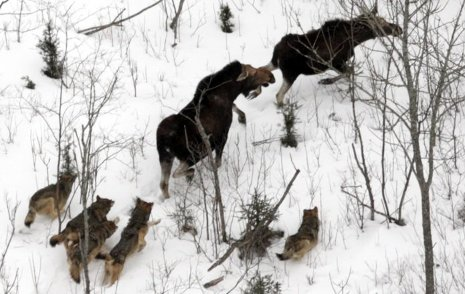
\includegraphics[height=5cm,keepaspectratio]{figs/isle-royale1} \\
%    }
%    \vfill
%    { \Large February 11 \& 13, 2019} \\
  \end{center}
\end{frame}




\section{Introduction}


%% \begin{frame}[plain]
%%   \frametitle{Today's topics}
%% %  {\huge Today's topics}
%%   \tableofcontents%[currentsection]
%% \end{frame}


\begin{frame}
  \frametitle{Introduction}
  \large
  \begin{itemize}%[<+->]
    \item<1-> Lotka and Volterra developed models for both predator-prey
      dynamics and competitive interactions.
    \item[]
    \item<2-> As usual, these models were developed as
      continuous-time models.
    \item[]
    \item<3-> We will focus on discrete-time versions ($t = 1, 2, \ldots$).
    \item[]
    \item<4-> We will ignore potential extensions with stochasticity, age
      structure, spatial structure, etc\dots
  \end{itemize}
\end{frame}


\section{Predator-Prey}



\begin{frame}
  \frametitle{Question}
  \Large
  How should predator-prey dynamics operate? \\
  \pause
  \vspace{1cm}  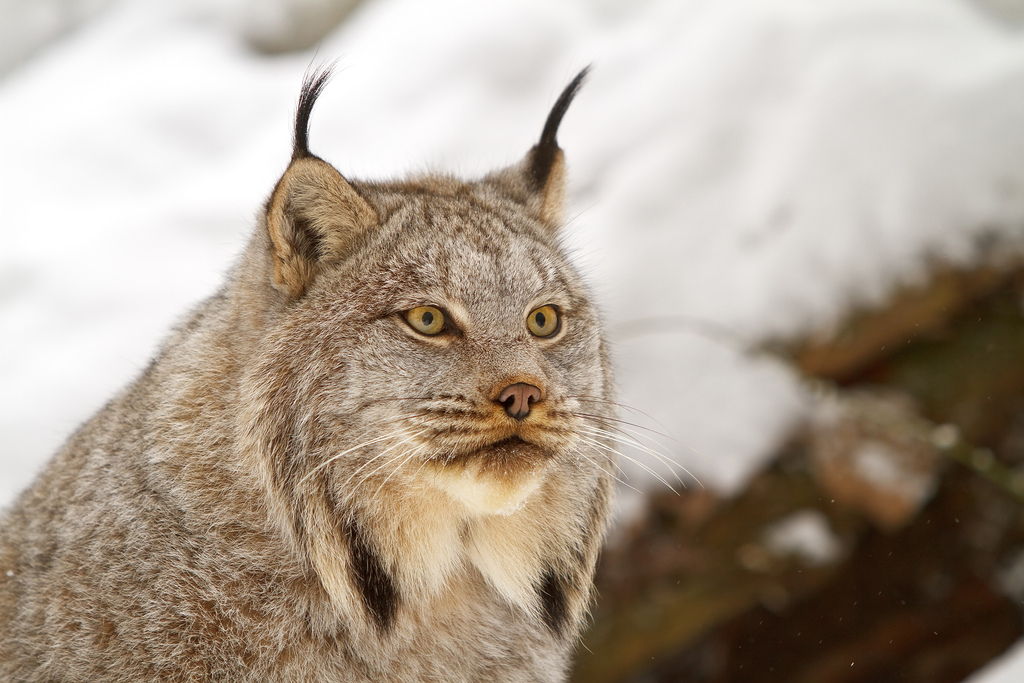
\includegraphics[height=4cm,keepaspectratio]{figs/Canada_lynx_portrait_by_Michael_Zahra} \hfill
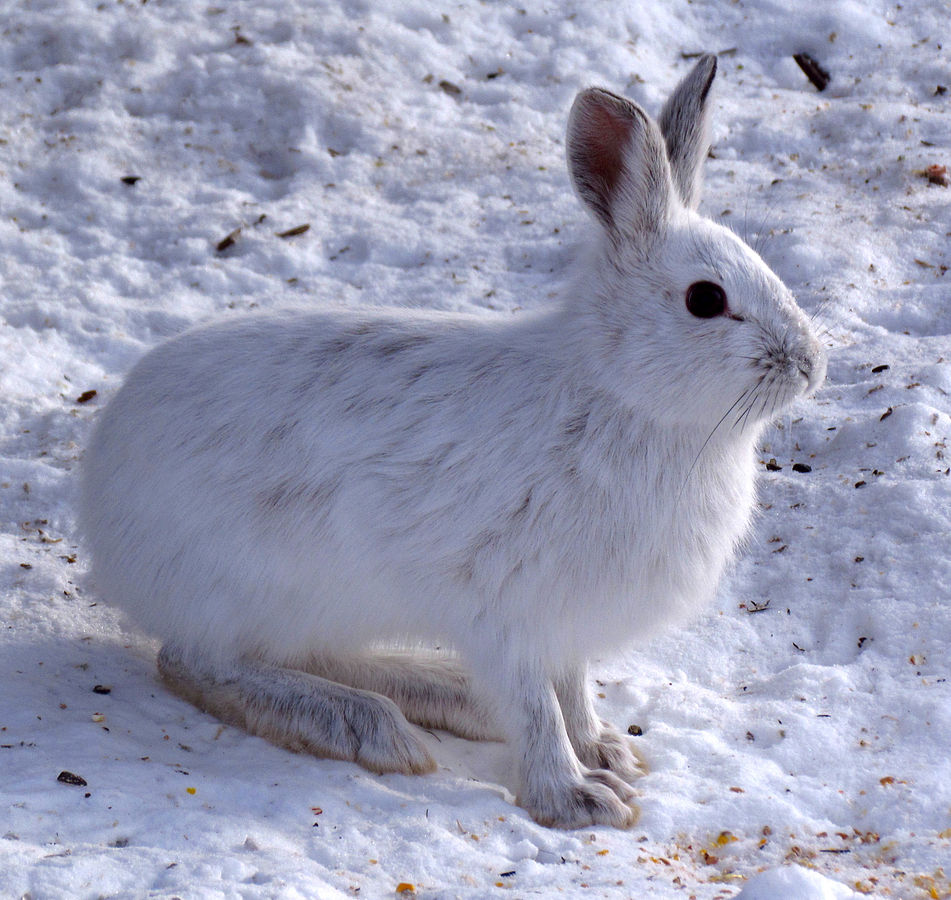
\includegraphics[height=4cm,keepaspectratio]{figs/Snowshoe_Hare,_Shirleys_Bay}
\end{frame}


%\begin{frame}
%  \frametitle{Paramecium}
%\end{frame}


\begin{frame}
  \frametitle{Lynx-hare cycles}
  \centering
  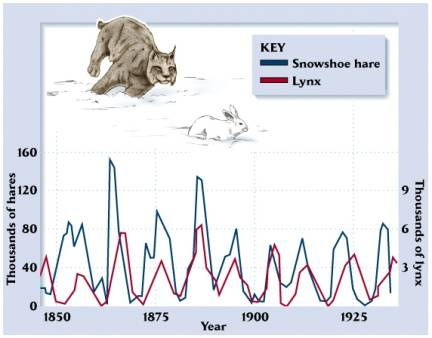
\includegraphics[width=0.75\textwidth]{figs/lynx-hare} \par
%  \includegraphics[width=0.8\textwidth]{figs/lynx-hare_cycle} \par
%  \small
%  \url{http://www.youtube.com/watch?v=t43Li0dLkvw}
\end{frame}







\begin{frame}
  \frametitle{Lotka-Volterra predator-prey model}
  \Large
  Model for prey
  \[
    N^{prey}_{t+1} = N^{prey}_t + N^{prey}_t (r^{prey} - d^{prey} N^{pred}_t)
  \] \\
  \vspace{1cm}
  \pause
  Model for predator
  \[
    N^{pred}_{t+1} = N^{pred}_t + N^{pred}_t (b^{pred}N^{prey}_t - d^{pred})
  \]
  \pause
  \vfill
  \normalsize
  \begin{itemize}
    \item Model is based on geometric growth
    \item $r^{prey}$ is the growth rate of the prey in the absence of
      predators
    \item $d^{prey}$ is the predation rate
    \item $b^{pred}$ is the birth rate of the predators
    \item $d^{pred}$ is the mortality rate of the predator
  \end{itemize}
\end{frame}



\begin{frame}
  \frametitle{Equilibrium}
  \Large
  Equilibrium for prey occurs when\dots
  \[
    N^{pred} = \frac{r^{prey}}{d^{prey}}
  \] \\
  \vspace{1cm}
  \pause
  Equilibrium for predators occurs when\dots
  \[
    N^{prey} = \frac{d^{pred}}{b^{pred}}
  \]
  \pause
  \vfill
  \large
  However, it is rare that both equilibrium conditions will be met at
  the same time, and so the populations will cycle.
\end{frame}



\begin{frame}[fragile]
  \frametitle{Model predicts population cycles}
\vspace{-1.2cm}

\begin{center}
  \includegraphics[width=\textwidth]{figure/predprey1-1}
\end{center}
\end{frame}





\begin{frame}
  \frametitle{Isle Royale wolves and moose}
  \centering
  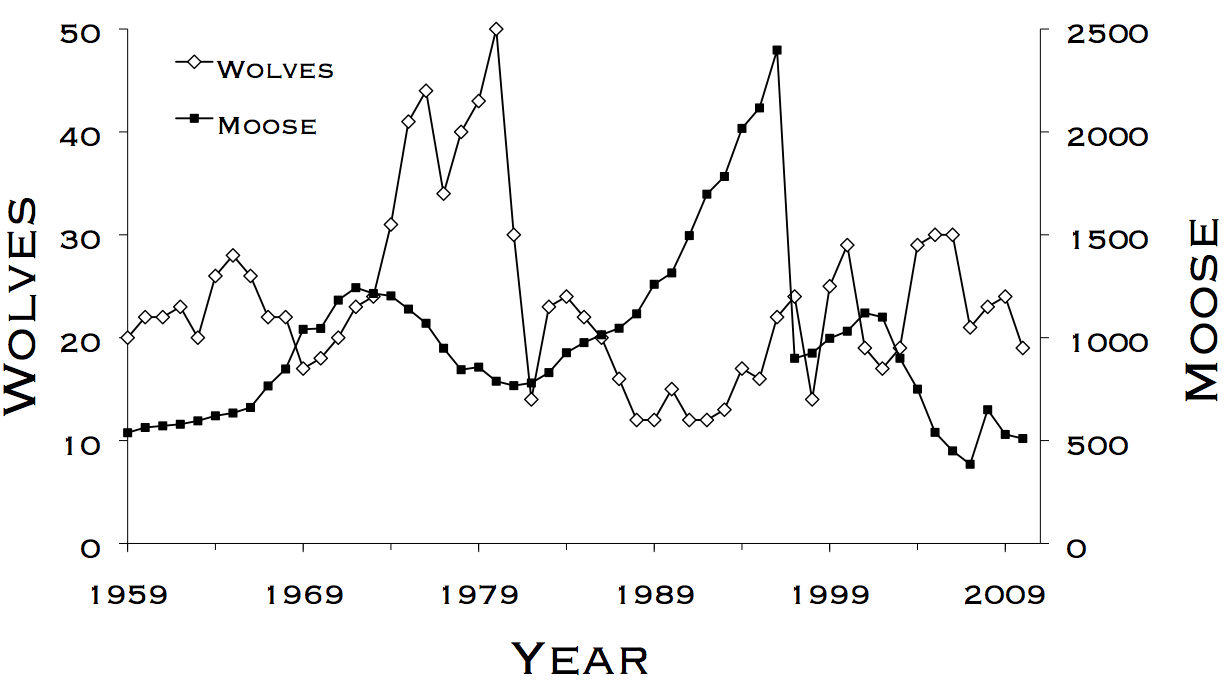
\includegraphics[width=1\textwidth]{figs/Fig01_wolfmoosechronology} \par
%  \url{http://www.youtube.com/watch?v=PdwnfPurXcs}
%  \url{http://vimeo.com/15411376}
  \url{https://youtu.be/PdwnfPurXcs}
%  \pause
%  Attack video: \url{https://youtu.be/Ju3er3xIl7E}
\end{frame}






\section{Competition}




\begin{frame}
  \frametitle{Competition}
  \begin{center}
    \includegraphics[width=.95\textwidth]{figs/Hyena_lion} \par
    \vspace{-0.5cm} \hspace{.75\textwidth}
    {\tiny David Bygott \par}
  \end{center}
%  \pause
%  \large
%  \begin{itemize}
%    \item Models are based on logistic growth
%    \item Usually applied to inter-specific competition
%  \end{itemize}
\end{frame}


\begin{frame}
  \frametitle{Lotka-Volterra competition model}
  \Large
  Model for species A
  \[
    N^A_{t+1} = N^A_t + r^A N^A_t(K^A - N^A_t - \alpha^B N^B_t) / K^A
%    N^A_{t+1} = N^A_t + r^A N^A_t\left(1-\frac{N^A_t - \alpha^B N^B_t}{K^A}\right)
  \] \\
  \vfill %\vspace{1cm}
  \pause
  Model for species B
  \[
    N^B_{t+1} = N^B_t + r^B N^B_t(K^B - N^B_t - \alpha^A N^A_t) / K^B
%    N^B_{t+1} = N^B_t + r^B N^B_t\left(1-\frac{N^B_t - \alpha^A N^A_t}{K^B}\right)
  \]
  \pause
  \vfill
%  \large
  \normalsize
  \begin{itemize}
  \item Model based on logistic growth
  \item The $\alpha$ parameters are competition coefficients
    determining how strongly each species affects the other
  \end{itemize}
\end{frame}



\begin{frame}
  \frametitle{Equilibrium}
  \Large
  Equilibrium for species A
  \[
    N^A = \frac{K^A - \alpha^B K^B}{1 - \alpha^A \alpha^B}
  \] \\
  \vspace{1cm}
  \pause
  Equilibrium for species B
  \[
    N^B = \frac{K^B - \alpha^A K^A}{1 - \alpha^A \alpha^B}
  \]
\end{frame}


\begin{frame}
  \frametitle{Three possible outcomes}
%  \Large
  \large
%  \begin{block}{Outcomes depend on the sign of the numerators}
  {\bf Outcomes depend on the sign of the numerators}
  \begin{enumerate}[(1)]
    \item Stable coexistence
    \item Competitive exclusion
    \item Unstable equilibrium
  \end{enumerate}
%  \end{block}
  \pause
  \vfill
%  \begin{block}{Competitive exclusion principle}
    \large %\normalsize
    {\bf Competitive exclusion principle}:
    Two species with the same niche cannot coexist on the same limiting resource
%  \end{block}
\end{frame}


%% \begin{frame}
%%   \frametitle{Competitive exclusion principal}
%%   \large
%%   \begin{center}
%%     Two species cannot coexist on the same limiting resource
%%     %unless their niches are sufficiently
%%     %different that each limits its own population growth more than it
%%     %limits that of the other
%%   \end{center}
%% \end{frame}




\begin{frame}
  \frametitle{Outcomes}
%  \frametitle{Competitive exclusion}
  \vspace{-1cm}


\begin{columns}
  \column{\dimexpr\paperwidth-10pt}
%  \begin{center}
    \includegraphics[width=0.49\textwidth]{figure/stable-1}
    \includegraphics[width=0.49\textwidth]{figure/compex-1}
%  \end{center}
\end{columns}
\end{frame}


\begin{frame}
  \frametitle{Don't forget about intraspecific competition}
  \centering 
  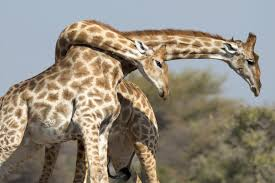
\includegraphics[width=0.8\textwidth]{figs/giraffe} \\
  \url{https://youtu.be/KQLPL1qRhn8}
\end{frame}


\begin{frame}
  \frametitle{Summary}
  \large
%  \begin{itemize}
%  \item<1->
  Predator-prey model is extension of geometric growth
    \begin{itemize}
      \item Predators and prey limit each other's growth potential
    \end{itemize}
%  \item[]
%  \item<2->
    \pause \vfill
    Competition model is extension of logistic growth
    \begin{itemize}
      \item Competitors influence each other's density-dependent
        regulation process
    \end{itemize}
%  \item[]
%  \item<3->
    \pause \vfill
    These models could be extended to include:
    \begin{itemize}%[<+->]
    \item More species
    \item Stochasticity
    \item Age structure
    \item Harvest
    \item Spatial structure
    \item Additional forms of density dependence
    \end{itemize}
%  \end{itemize}
\end{frame}




%% \begin{frame}
%%   \frametitle{Assignment}
%%   \huge
%%   Read
%% \end{frame}



%% \begin{frame}
%%   \frametitle{Assignment}
%%   Read this article on the Isle Royale wolves and moose:
%%   \url{http://www.isleroyalewolf.org/http\%3A//www.cpc.ncep.noaa.gov/products/precip/CWlink/pna/nao.shtml}
%% \end{frame}



%% \section{FL panther}



%% \begin{frame}
%%   \frametitle{Florida panther and white-tailed deer}
%%   \begin{center}
%%     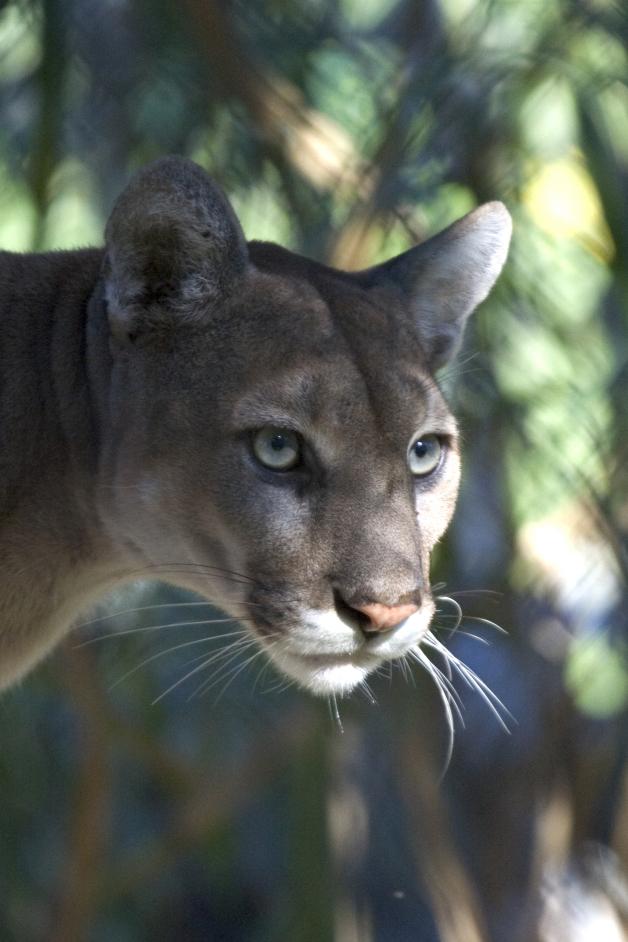
\includegraphics[height=5.3cm,keepaspectratio]{figs/panther1} \hfill
%%     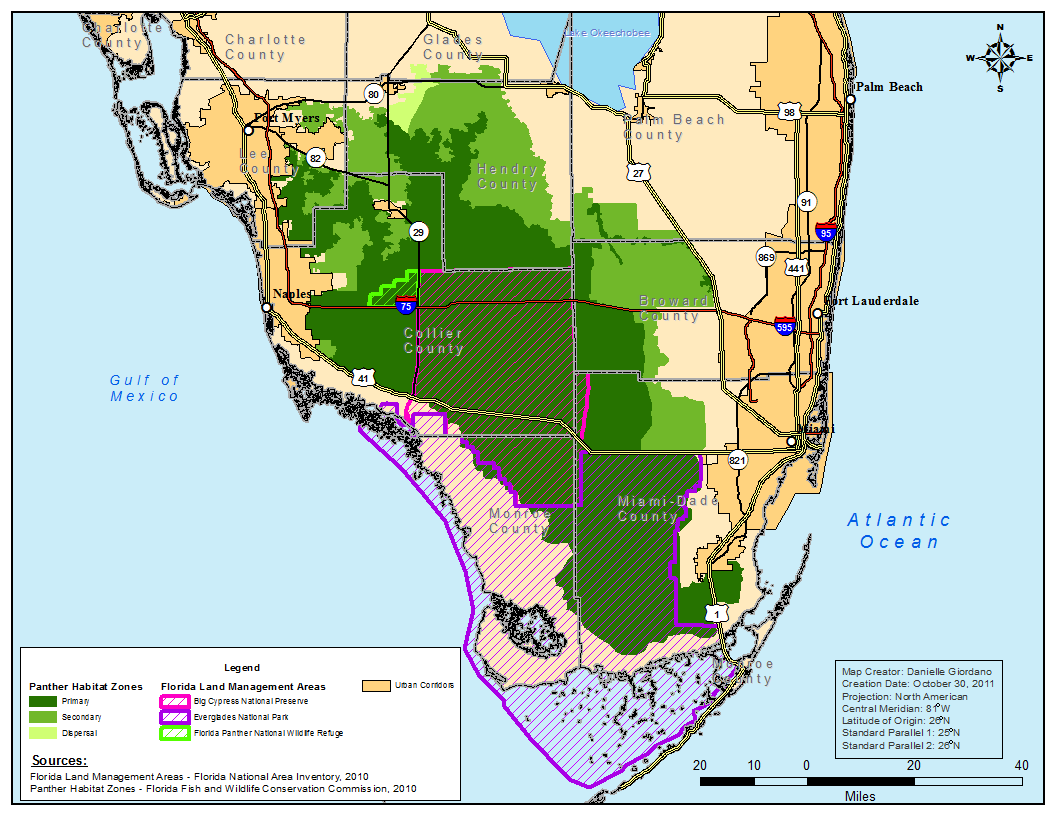
\includegraphics[height=5.3cm,keepaspectratio]{figs/FloridaPantherHabitat}
%%   \end{center}
%% \end{frame}


%% \begin{frame}
%%   \frametitle{Motivation}
%%   {\centering \bf %Problem \\}
%%   FL panther is endangered but populations have increased %rapidly
%%   since introduction of Texas cats \par}
%% \begin{center}
%%   \fbox{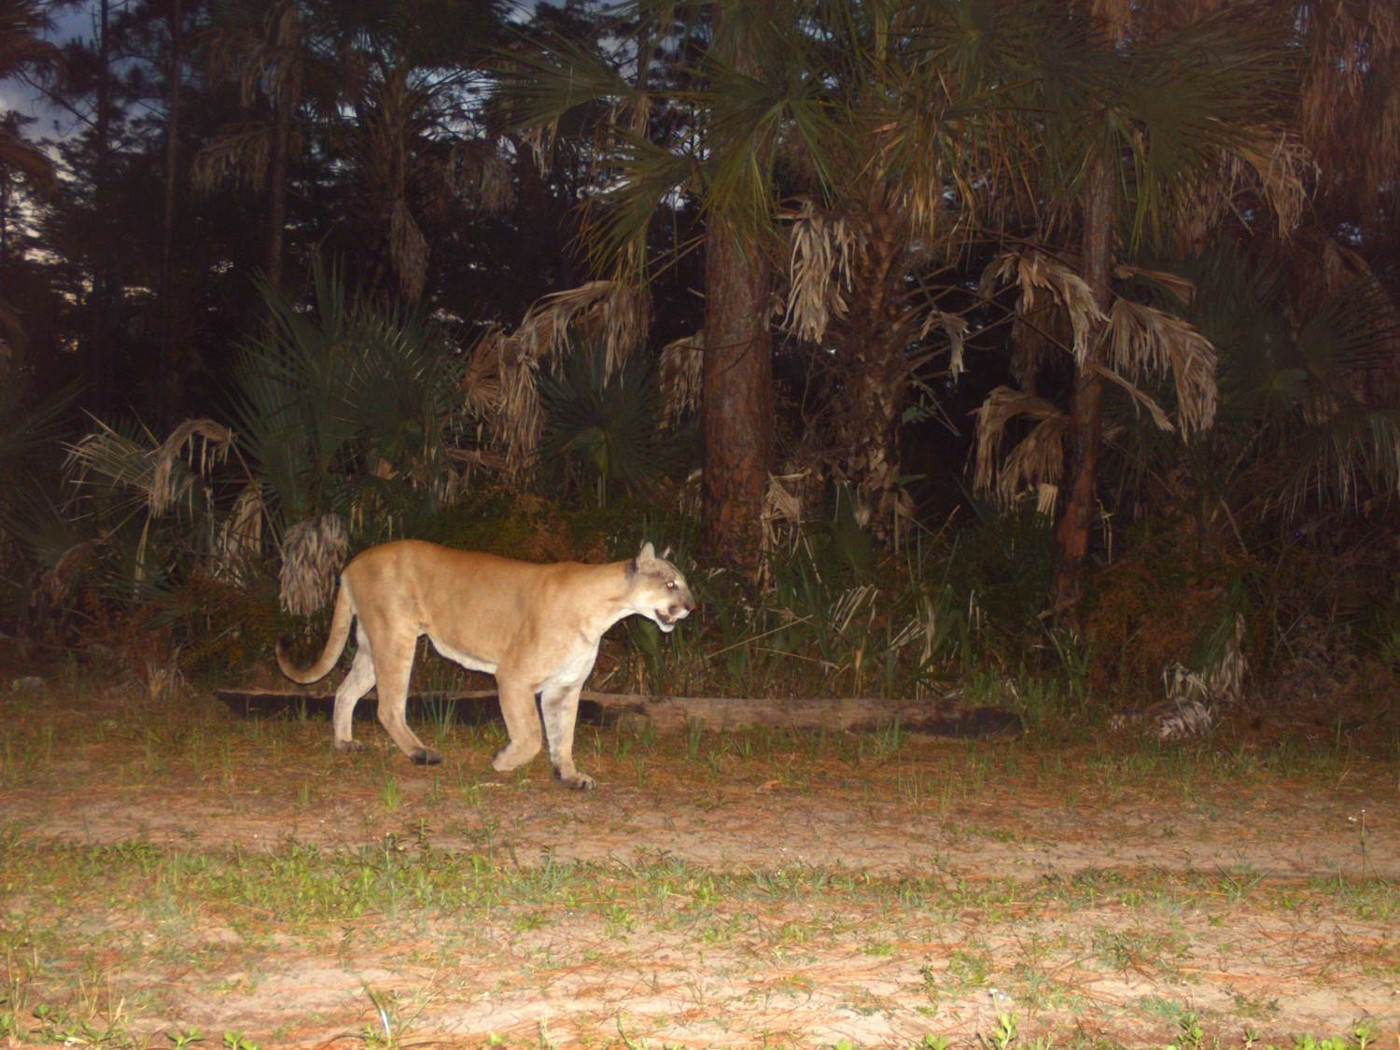
\includegraphics[height=3.7cm,keepaspectratio]{figs/pantherCamera}} \hfill
%%   \fbox{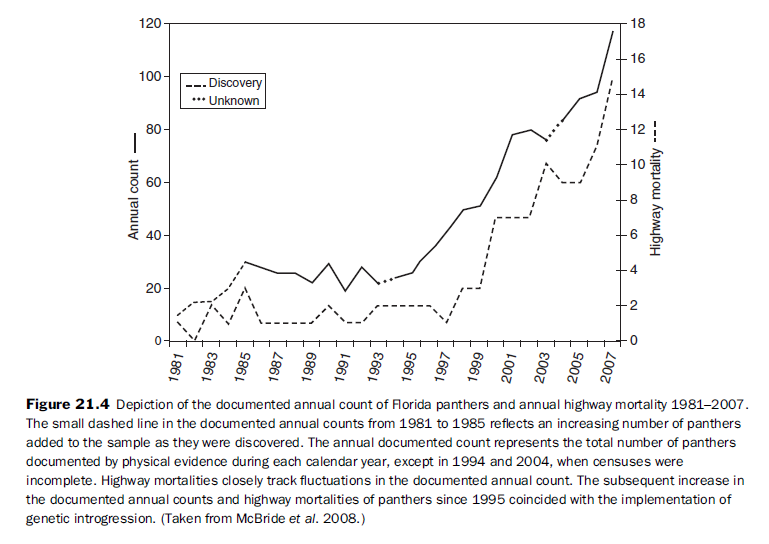
\includegraphics[height=3.7cm,keepaspectratio]{figs/pantherTrend}}
%% \end{center}
%% \end{frame}




%% \begin{frame}
%%   \frametitle{Motivation}
%%   {\centering \bf Prey populations appear to be declining rapidly, perhaps in
%%     response to panthers \par}
%%   \pause
%%   \begin{center}
%%     Feral pigs are almost gone in some areas
%%     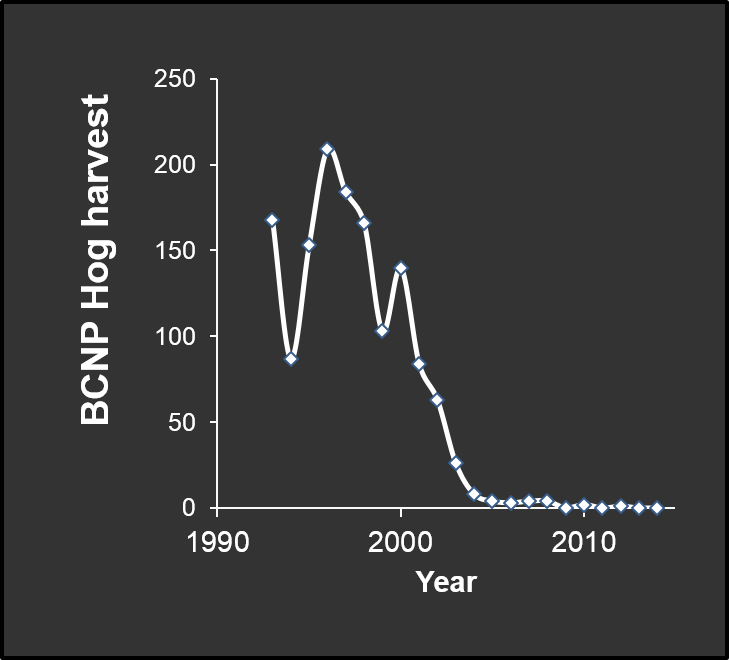
\includegraphics[width=0.6\textwidth]{figs/hogHarvest}
%%   \end{center}
%% \end{frame}



%% \begin{frame}
%%   \frametitle{Motivation}
%%   {\centering \bf     Deer numbers are also down in some regions \par}
%% %Prey populations appear to be declining rapidly, perhaps in
%% %    response to panthers}
%%   \begin{center}
%%     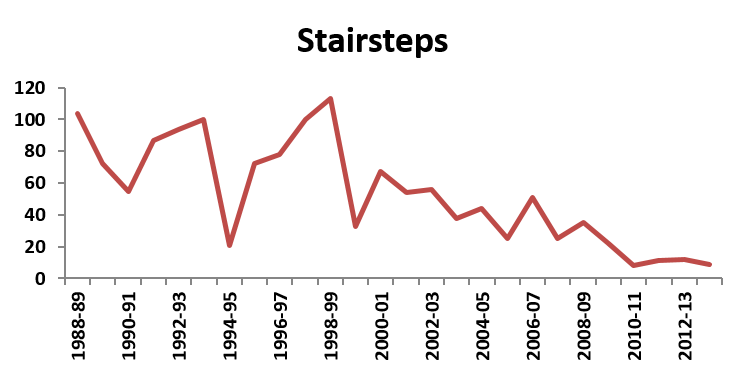
\includegraphics[width=\textwidth]{figs/deerStairsteps}
%%   \end{center}
%% \end{frame}



%% \begin{frame}
%%   \frametitle{Motivation}
%%   \large
%%   {\bf Concerns}
%%   \begin{itemize}[<+->]
%%     \item Loss of prey base could force panthers into developed areas
%%     \item Rate of human-panther encounters is on the rise
%%     \item Numerous reports of pet and livestock losses
%%   \end{itemize}
%% \end{frame}




%% %% \begin{frame}
%% %%   \frametitle{UGA deer study}
%% %%   \large
%% %%   {\bf Research questions \\}
%% %%   \begin{itemize}
%% %%     \item Can the deer population sustain increasing panther population?
%% %%     \item Can the deer population sustain ongoing hunting?
%% %%     \item How will changes in hydrology affect deer populations?
%% %%   \end{itemize}
%% %%   \begin{center}
%% %%     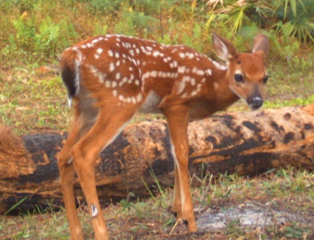
\includegraphics[height=2.5cm,keepaspectratio]{figs/fawn} \hfill
%% %%     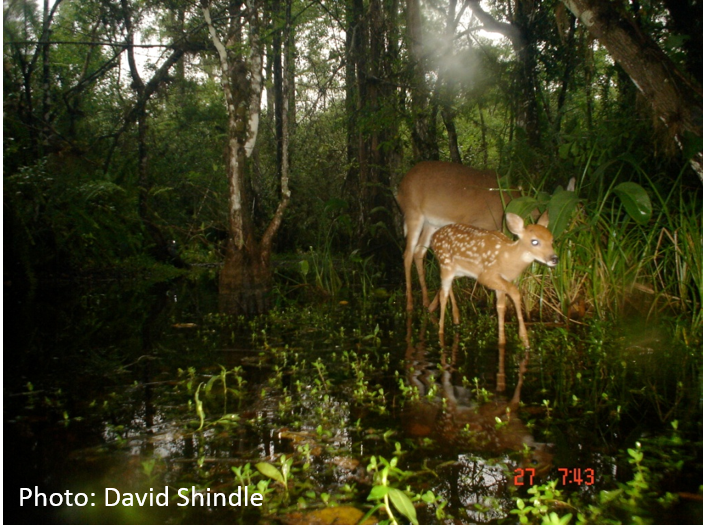
\includegraphics[height=2.5cm,keepaspectratio]{figs/deerCamera} \hfill
%% %%     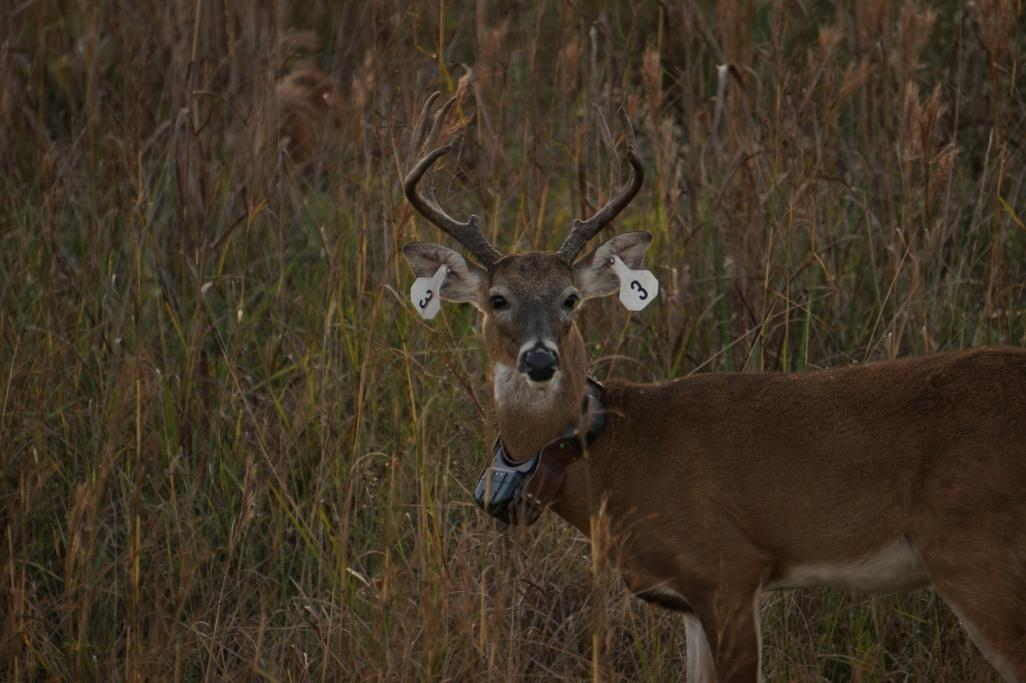
\includegraphics[height=2.5cm,keepaspectratio]{figs/deer_collar}
%% %%   \end{center}
%% %% \end{frame}




%% \begin{frame}
%%   \frametitle{In-class exercise}
%%   \large
%%   {\bf Break into groups of 4-5 and answer the following: \par}
%%   \begin{enumerate}[\bf (1)]
%%     \item Do you think panthers are likely to elimanate the deer
%%       population in South Florida? Why or why not?
%%     \item How could you use or modify the Lotka-Volterra model to
%%       address this question?
%% %    \item How would you determine if panthers are likely to decimate
%% %      deer population?
%%     \item What factors other than panthers might determine future deer
%%       numbers?
%%   \end{enumerate}
%%   \begin{center}
%%     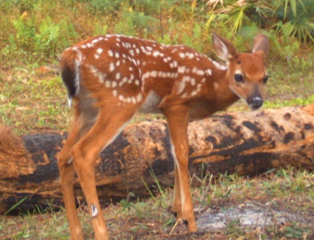
\includegraphics[height=2.5cm,keepaspectratio]{figs/fawn} \hfill
%%     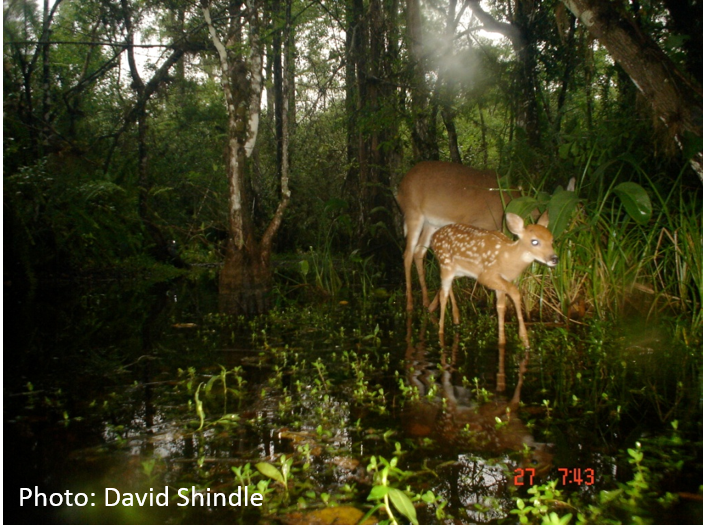
\includegraphics[height=2.5cm,keepaspectratio]{figs/deerCamera} \hfill
%%     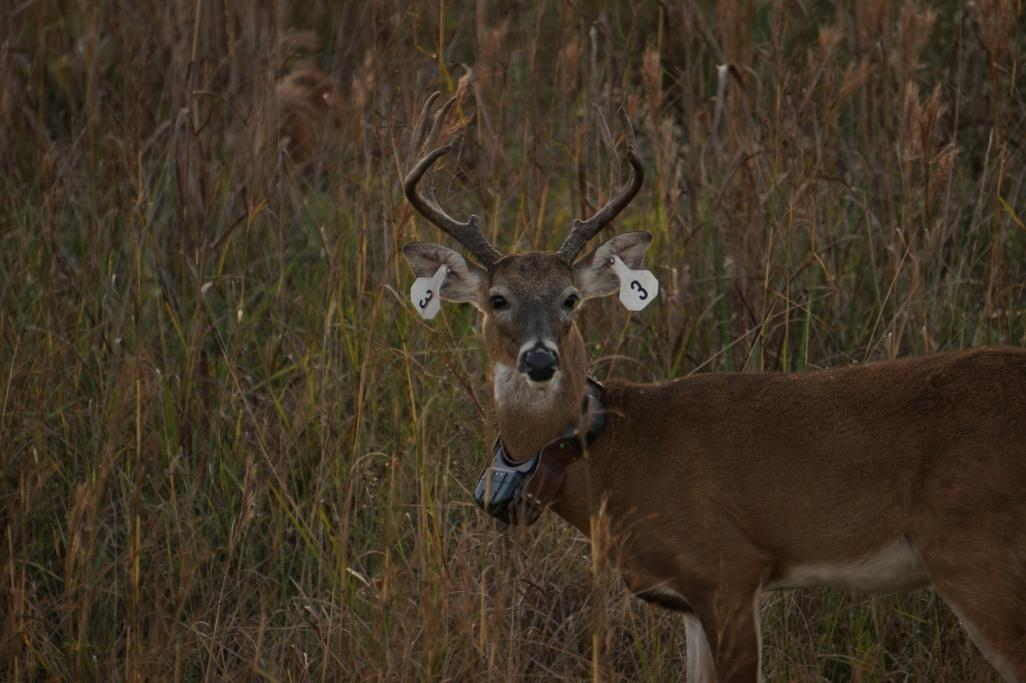
\includegraphics[height=2.5cm,keepaspectratio]{figs/deer_collar}
%%   \end{center}
%%   \note{Potential answers:
%%     We need to understand spatial and temporal variation in vital rates

%%     Is predation rate higher than prey birth rate

%%     Does the deer growth rate increase when numbers are low? Is there
%%     density dependence

%%     Are there refugia where deer can persist? Is there a human
%%     shielding effect?
%%     }
%% \end{frame}





%% \begin{frame}
%%   \frametitle{Theory}
%%   Models
%% \end{frame}


%% \begin{frame}
%%   \frametitle{Theory}
%%   Hutchinson's lab experiements

%%   Importance of space / refugia / mortality rate of predators
%% \end{frame}


%% \begin{frame}
%%   \frametitle{Theory}
%%   Spatial variation in vital rates
%% \end{frame}



%% \begin{frame}
%%   \frametitle{Objectives}

%% \end{frame}







\end{document}


